\newcommand{\latticeHead}{latticeTop} 
\newcommand{\securityClass}{SC}
\newcommand{\liberalStar}{\textit{liberal $\star$-property}}
\newcommand{\strictStar}{\textit{strict $\star$-property}}
%\subsection{LBAC in \labacOneOneOne} 




LBAC or Lattice Based Access Control is characterized by one directional information flow in a lattice of security classes. The security classes are partially ordered. One security class from these classes is assigned to each user which is known as clearance of the user. A user having a senior security class can also exercise his/her privileges using a junior  security class. For example, a top secret user can also exercise his privileges as secret user but he/she cannot use both secret and top secret clearance at the same time.  On the other hand, one security class (from the same classes of the security lattice) is assigned on objects commonly known as classification of the object. LBAC enforces one direction of information flow by two mandatory rules for reading and writing of these objects. One rule, known as \textit{simple-security property} (informally, read down rule), states that a subject (or user) can read an object if subject's clearance dominates object's classification. The other rule, known as \textit{liberal $\star$-property} (informally, write up rule),  states that a subject can write on an object if object's classification dominates subject's clearance. As a security class dominates itself it is possible to read and write  at the same level. A variation of \textit{liberal $\star$-property}, know as \textit{strict $\star$-property}, mandates that a subject can only write at his own level for the purpose of integrity requirements. A definition of LBAC is given in Segment I of Table \ref{tab:lbac-in-labac}.

\newcommand{\userLBAC}{U_{L}}
\newcommand{\objectLBAC}{O_{L}}
\newcommand{\sessionLBAC}{S_{L}}
\newcommand{\sessionUser}{sub\_creator}
\newcommand{\clearance}{clearance}
\newcommand{\classification}{classification}

\begin{table}
	\centering
	\caption{ LBAC in \labacOneOneOne{}} %\vspace*{3pt}
	\label{tab:lbac-in-labac}
	\begin{tabular}{|l|}						
		\hline					
		\multicolumn{1}{|c|}{\underline{\textit{I. LBAC components }}}\\	\\			 
		 - $\userLBAC, \objectLBAC$ and $\sessionLBAC$ (set of users, objects and sessions resp.) \\
		 -  \textit{SC}:  set of security classes in the lattice \\
		 -  \textit{SCH}: partial order on \textit{SC} (also denoted by $\succeq$ ) \\
		 - $\sessionUser: \sessionLBAC \to \userLBAC$, many-to-one mapping  from $\sessionLBAC$ to $\userLBAC$\\
		 - $\clearance: (\userLBAC \cup \sessionLBAC) \to SC$,  and  $clearance(s) \preceq \clearance(\sessionUser(s))$\\
		 - $\classification: \objectLBAC \to SC$\\		
	
		 - \textit{Simple-security property}: Subject s can read object o \\ \hfill only if \textit{clearance(s) $\succeq$ classification(o)}\\
		 - \textit{Liberal $\star$-property}: Subject s can write object o\\ \hfill only if  \textit{clearance(s) $\preceq$ classification(o)}\\
		  - \textit{Strict $\star$-property}: Subject s can write object o\\ \hfill only if  \textit{clearance(s) = classification(o)}\\
%		  - $createSession(u:\userLBAC,s:\sessionLBAC, sc:SC)$ \\ \hfill condition:$ s \not \in \sessionLBAC \land \clearance(u) \succeq sc$ \\ \hfill \hfil update: $\sessionLBAC' = \sessionLBAC \cup s$\\
		  
		  	\\	  \multicolumn{1}{|c|}{\underline{\textit{II. Construction in \labacOneOneOne{} }}} \\ \\
		  
		\\	  \multicolumn{1}{|l|}{{\textit{II(a). Construction of basic sets and relations }}} \\
		 - $U = \userLBAC, O = \objectLBAC, S = \sessionLBAC, A=\{read, write\}$\\
		 
		 - $\creator(s) = \sessionUser(s)$, for $s \in S$\\
		 -  $UL = SC,  ULH = SCH$ \\
		 - $OL = \{sc | sc \in SC \} \cup \{sc' | sc \in SC \}$\\
		 - $OLH=\{ (sc_i, sc_j) | sc_i \succeq sc_j \} \cup \{ (sc_i', sc_j') | sc_j' \succeq sc_i'\} $  [\liberalStar{}]\\
		 - $OLH=\{ (sc_i, sc_j) | sc_i \succeq sc_j \} $  [\strictStar{}]\\
		 -  $  \uLabel(u) =  clearance(u)$ \\
		 -  $  \oLabel(o) =  \{ sc, sc'\}$, where $sc=\classification(o)$	\\
		 - $ \Policy_{read} = \{ (sc_i, sc_i)| sc_i \in SC \}$ \\
		 - $ \Policy_{write} = \{ (sc_i, sc_i')| sc_i \in SC  \}$ \\
		% - Def. of  $\impliedPolicy_{op_i}$,  $\sessionLabels(s)$ for session $s \in S$ \\ \hfill and $\request(s, a, o)$  are unchanged from Table \ref{tab:labac-definition}	\\	
		 %- Session Constraints: $|\sessionLabels(s)  \cap SC| = 1$
		 
		 \\ \multicolumn{1}{|l|}{{\textit{II(b). Condition on session functions}}} \\ \\
		 - $f_{\createSession} (u, s, val) : |val|=1$\\
		 - $f_{\deleteSession}(u,s): true$\\
	     - $f_{\assignValues} (u, s, val): false$ [assuming tranquility]\\
	     - $f_{\removeValues} (u, s, val): false$ [assuming tranquility]\\
	     
	     \\ \multicolumn{1}{|c|}{\underline{\textit{III. LaBAC extension for object creation}}} \\
	     - $\createObject(s,o,\{val\})$: create a new object, and    assign value $\{val\}$\\
		    \hspace{5em} condition: $s \in S \land o \not \in O \land \exists ul  \in \sessionLabels(s)  $  $ \land val \succeq ul]$ \\
		      \hspace{5em} update: $O' = O \cup \{o\}, \oLabel(o) = \{val\}$ \\
%		 - $\updateObject(s,o,\{val\})$: update $\oLabel$ value \\ \hfill of existing object\\
%		 \hfil condition: $s \in S \land o \in O \land \exists ol, \exists ul [\sessionLabels(s)=ul \land$ \\ \hfill $  \oLabel(o) = ol \land ul \udominate ol \land ul \udominate val ]$ \\
%		   \quad  update: $ \oLabel(o) = \{val\}$ 
	 \hline	
	\end{tabular}	
\end{table}



 

We present the configuration of LBAC in  \labacOneOneOne{}. Minimalistically, we need \consLabac{}  to configure some constraints of LBAC, for example, at most one security class can be activated by a subject (i.e. session in case of \eapABAC{} ) at a time. We use \labacOneOneOne{} for convenience.  

 The configuration of LBAC in \labacOneOneOne{} is given in Segment II of Table \ref{tab:lbac-in-labac}.  The security classes and its hierarchy are directly used as user label values and its hierarchy. For object-label values and its hierarchy we consider both the original lattice and the inverted lattice. The clearance of a user in LBAC  is assigned as $\uLabel$ values of the user in \eapABAC{} . On the other hand, if an object has a classification of $sc \in SC$ in LBAC,  we assign the object $\oLabel$ values of \{\textit{sc,sc'}\}, where $sc'$ correspond to $sc$ in the inverted lattice.  The \textit{simple-security} property is configured as a \eapABAC{}  policy  $\Policy_{read} \equiv \{(sc_i, sc_i)\}$ so that users having user-label value $sc_i$ can read objects having object-label value $sc_i$ or its junior.  Similarly, the $\star$-\textit{property} is configured with $\Policy_{write} \equiv \{(sc_i, sc_i')\}$ where $sc_i$ is the user-label value from the original lattice and $sc_i'$ is the object-label value from the inverted lattice and  $sc_i$  correspond to $sc_i'$. For the \liberalStar, we consider the hierarchy of the inverted lattice where as we do not consider them for the \strictStar.  An example of LBAC configured in \labacOneOneOne{} is given in Figure \ref{fig:lbac-labac-example}.

 \begin{figure}
 	\centering
 	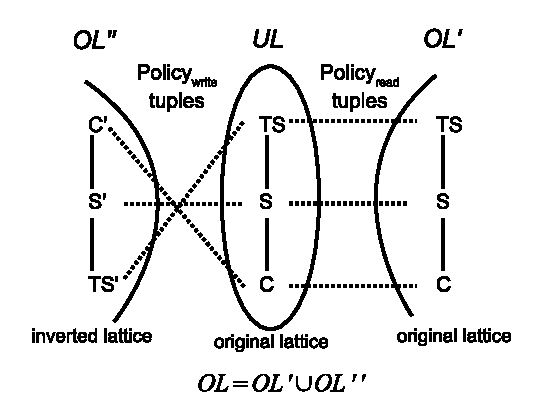
\includegraphics[width=.4\textwidth]{ABAC16/lbac-labac-example}
 	\caption{LBAC example configured in LaBAC}
 	\label{fig:lbac-labac-example}
 \end{figure}
\begin{table} 
	\centering
 \caption{Quantifying \eapABAC{} for simulating LBAC}
 \label{tab:lbac-labac-quantification}
	\begin{tabular}{|l|}
		\hline	                                                                                                           	

		$|UL| = |SC|$ and $|OL| =  2 |SC|  $\\
		$|\Policy| = 2$  $(|\Policy_{read}| $ and $|\Policy_{write}|)$\\
		%|\policy_{read}| =  1$\\
		%|\policy_{write}| =  1$\\
		\hline
		\end{tabular}  

\end{table}

Segment II(b) of Table \ref{tab:lbac-in-labac} specifies conditions for the session management functions in \eapABAC{} . In  $\createSession()$ we specify additional condition so that at most one user-label value can be activated in one session. We assume, once created clearance of subjects and classification of objects cannot be changed. This property in known \textit{tranquility} in the literature \cite{lbac}
  
Segment III is an extension of \labacOneOneOne{} for the purpose of creating objects in \eapABAC{} . Since functional specification of \labacOneOneOne{} does not include functions for creating or managing objects,  here we define a function $\createObject()$ for this purpose. We follow the \liberalStar{} as the precondition for creation of objects. 

%and $\updateObject()$ to capture creation of new objects and modification of object classification values in LBAC. The prerequisite conditions and necessary updates for execution of these functions are also presented here. 


Finally, Table \ref{tab:lbac-labac-quantification} shows required number of authorization policies, $UL$ and $OL$ values  for configuring LBAC.

%to configure LBAC in \labacOneOneOne{}.

%we quantify required number of required \labacOneOneOne{} policies for configuring LBAC which is shown in Table \ref{tab:lbac-labac-quantification}. As we can see, we need as many read and write policies as the number of security classes in the lattice.



 
